\documentclass[12pt]{article}
\usepackage{tikz}

\begin{document}

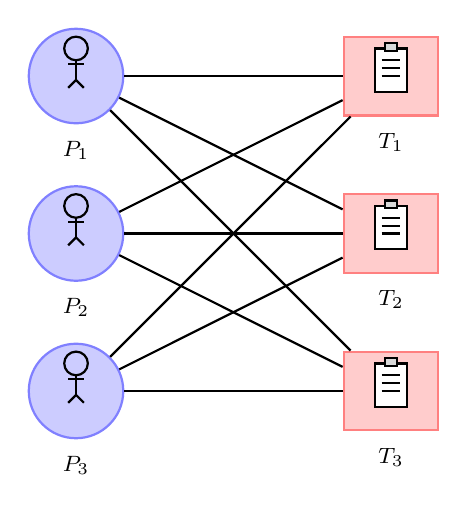
\begin{tikzpicture}[
    every node/.style={font=\footnotesize},
    person/.style={circle, draw=blue!50, fill=blue!20, thick, minimum size=1.2cm},
    task/.style={rectangle, draw=red!50, fill=red!20, thick, minimum width=1.2cm, minimum height=1cm},
    % Define a stick figure pic
    pics/stickfigure/.style={
        code={
            \draw[thick] (0,0.2) circle (0.15); % Head
            \draw[thick] (0,0.05) -- (0,-0.2);  % Body
            \draw[thick] (-0.1,-0.3) -- (0,-0.2) -- (0.1,-0.3); % Legs
            \draw[thick] (-0.1,0) -- (0.1,0);   % Arms
        }
    },
    % Define a clipboard pic
    pics/clipboard/.style={
        code={
            \draw[thick, fill=white] (-0.2,-0.3) rectangle (0.2,0.25); % Clipboard body
            \draw[thick, fill=gray!30] (-0.08,0.22) rectangle (0.08,0.32); % Clip
            \draw[thick] (-0.12,0.1) -- (0.12,0.1); % Line 1
            \draw[thick] (-0.12,0) -- (0.12,0);    % Line 2
            \draw[thick] (-0.12,-0.1) -- (0.12,-0.1); % Line 3
        }
    }
]

% Nodes for people (with stick figures drawn via pic)
\node[person] (P1) at (0, 2) {};
\pic at (0, 2.15) {stickfigure};
\node[below=0.05cm] at (0, 1.35) {$P_1$};

\node[person] (P2) at (0, 0) {};
\pic at (0, 0.15) {stickfigure};
\node[below=0.05cm] at (0, -0.65) {$P_2$};

\node[person] (P3) at (0, -2) {};
\pic at (0, -1.85) {stickfigure};
\node[below=0.05cm] at (0, -2.65) {$P_3$};

% Nodes for tasks (with clipboard symbols drawn via pic)
\node[task] (T1) at (4, 2) {};
\pic at (4, 2.1) {clipboard};
\node[below=0.05cm] at (4, 1.45) {$T_1$};

\node[task] (T2) at (4, 0) {};
\pic at (4, 0.1) {clipboard};
\node[below=0.05cm] at (4, -0.55) {$T_2$};

\node[task] (T3) at (4, -2) {};
\pic at (4, -1.9) {clipboard};
\node[below=0.05cm] at (4, -2.55) {$T_3$};

% Edges (Complete bipartite graph)
\foreach \i in {1,2,3} {
    \foreach \j in {1,2,3} {
        \draw[thick] (P\i) -- (T\j);
    }
}

\end{tikzpicture}

\end{document}
